\documentclass[12pt]{article}

\setlength{\oddsidemargin}{0in}
\setlength{\textwidth}{6.5in}
\setlength{\topmargin}{-0.5in}
\setlength{\textheight}{9in}

%%%%%%%%%%%%%%%%%%%%%%%%%%%%%%%%%%%
%%%% General packages %%%%%
%%%%%%%%%%%%%%%%%%%%%%%%%%%%%%%%%%%

\usepackage{graphicx} % Include figure files
\usepackage{caption}
\usepackage{color} % Include colors for document elements
\usepackage{dcolumn} % Align table columns on decimal point
\usepackage{float}
\usepackage[hidelinks]{hyperref} % hidelinks added to not display red box for links
\usepackage{algorithm}
\usepackage{enumitem} % Necesarry for enumerating with romans (i), (ii), ...

%%%%%%%%%%%%%%%%%%%%%%%%%%%%%%%%%%%
%%%% Customized packages %%%%%
%%%%%%%%%%%%%%%%%%%%%%%%%%%%%%%%%%%

% Authors information
\usepackage{contributors}
% Julia code
\usepackage{jlcode}
% Math 
\usepackage{mymath}

%%%%%%%%%%%%%%%%%%%%%%%%%%%%%%%%%%%
%%%% Bibliography %%%%%
%%%%%%%%%%%%%%%%%%%%%%%%%%%%%%%%%%%

\usepackage[
backend=biber,
style=numeric, 
sorting=none
]{biblatex}

\addbibresource{bibliography.bib}

%%%%%%%%%%%%%%%%%%%%%%%%%%%%%%%%%%%
%%%% Document %%%%%
%%%%%%%%%%%%%%%%%%%%%%%%%%%%%%%%%%%

\title{A Review of Sensitivity Methods \\ for Differential Equations}

\date{\today}

\begin{document}
\maketitle

\hfill \break
\thanks
\newpage

% \begin{abstract}
The differentiable programming paradigm has become a central component of modern machine learning and scientific computing techniques. 
A long tradition of this paradigm exists in the context of scientific computing, in particular in differential equation-constrained, gradient-based optimization.
The recognition of the strong conceptual synergies between inverse methods and machine learning offers the opportunity to lay out a coherent framework applicable to both fields.
For models described by differential equations, the calculation of sensitivities and gradients requires careful algebraic and numeric manipulations of the underlying dynamical system.
Here, we provide a comprehensive review of existing techniques to compute derivatives of numerical solutions of differential equation systems.
We first discuss the importance of gradients of solutions of ODEs in a variety of scientific domains.
% , covering computational fluid dynamics, electromagnetism, geosciences, meteorology, oceanograpgy, climate science, flux inversion, glaciology, solid earth geophysics, biology and ecology, and quantum physics.
Second, we lay out the mathematical foundations of the various approaches and compare them with each other. 
Finally, we delve into the computational considerations and explore the solutions available in modern scientific software. 
% \end{abstract}

\normalsize

\clearpage

\tableofcontents
\clearpage

\section{Introduction}
% General statement: why gradients are important?
Evaluating how the value of a function changes with respect to its arguments and parameters plays a central role in optimization, sensitivity analysis, Bayesian inference, and uncertainty quantification, among many. 
Modern machine learning applications require the use of gradients to explore and exploit more efficiently the space of parameters. 
When optimizing a loss function, gradient-based methods (for example, gradient descent and its many variants \cite{ruder2016overview-gradient-descent}) are more efficient at finding a minimum and converge faster to them than gradient-free methods.
When numerically computing the posterior of a probabilistic model, gradient-based sampling strategies converge faster to the posterior distribution than gradient-free methods. 
Second derivatives further help to improve the convergence rates of these algorithms and enable uncertainty quantification around parameter values.
\textit{A gradient serves as a compass in modern data science: it tells us in which direction in the open wide ocean of parameters we should move towards in order to increase our chances of success}.  

% Differential Programming
Dynamical systems governed by differential equations are not an exception to the rule.
Differential equations play a central role in describing the behaviour of systems in natural and social sciences. 
Some authors have recently suggested differentiable programming as the bridge between modern machine learning methods and traditional scientific models \cite{Ramsundar_Krishnamurthy_Viswanathan_2021, Shen_diff_modelling, Gelbrecht-differential-programming-Earth}. 
Being able to compute gradients and sensitivities of dynamical systems opens the door to more complex models.
This is very appealing in geophysical models, where there is a broad literature on physical models and a long tradition in numerical methods. 
The first goal of this work is to introduce some of the applications of this emerging technology and to motivate its incorporation for the modelling of complex systems in the natural and social sciences. 
\begin{quote}
    \textbf{Question 1. }
    \textit{What are the scientific applications of differentiable programming for complex dynamical systems?}
\end{quote}

% Some examples
Sensitivity analysis corresponds to any method aiming to calculate how much the output of a function or program changes when we vary one of the model parameters. 
This task is performed in different ways by different communities when working with dynamical systems. 
In statistics, the sensitivity equations enable the computation of gradients of the likelihood of the model with respect to the parameters of the dynamical system, which can be later used for inference \cite{ramsay2017dynamic}. 
In numerical analysis, sensitivities quantify how the solution of a differential equation fluctuates with respect to certain parameters. 
This is particularly useful in optimal control theory \cite{Giles_Pierce_2000}, where the goal is to find the optimal value of some control (e.g. the shape of a wing) that minimizes a given loss function. 
In recent years, there has been an increasing interest in designing machine learning workflows that include constraints in the form of differential equations. 
Examples of this include Physics-Informed Neural Networks (PINNs) \cite{PINNs_2019} and Universal Differential Equations (UDEs) \cite{rackauckas2020universal}.  
Furthermore, numerical solvers are used as forward models in the case of Neural ordinary differential equations \cite{chen_neural_2019}.

% soft / hard constrains

% Differentiation 
However, when working with differential equations, the computation of gradients is not an easy task, both regarding the mathematical framework and software implementation involved. 
Except for a small set of particular cases, most differential equations require numerical methods to calculate their solution and cannot be differentiated analytically. 
This means that solutions cannot be directly differentiated and require special treatment if, besides the numerical solution, we also want to compute first or second-order derivatives. 
Furthermore, numerical solutions introduce approximation errors. 
These errors can be propagated and amplified during the computation of the gradient. 
Alternatively, there is a broad literature on numerical methods for solving differential equations. 
Although each method provides different guarantees and advantages depending on the use case, this means that the tools developed to compute gradients when using a solver need to be universal enough in order to be applied to all or 
at least to a large set of them. 
The second goal of this article is to review different methods that exist to achieve this goal.
\begin{quote}
    \textbf{Question 2. }
    \textit{How can I compute the gradient of a function that depends on the numerical solution of a differential equation?}
\end{quote}
%Notice here the phrase \textit{the gradient of a function that depends}, emphasizing the fact that in many cases we may be interested in computing the gradient of a function that depends on the solution of the differential equation.
%This is certainly the case in machine learning and optimization where the goal is to minimize a loss function that depends of some predicted and target responses. 

% AD
The broader set of tools known as Automatic Differentiation (AD) aims at computing derivatives by sequentially applying the chain rule to the sequence of unit operations that constitute a computer program. 
The premise is simple: every computer program, including a numerical solver, is ultimately an algorithm described by a chain of simple algebraic operations (addition, multiplication) that are easy to differentiate and their combination is easy to differentiate by using the chain rule. 
Although many modern differentiation tools use AD to some extent, there is also a family of methods that compute the gradient by relying on an auxiliary set of differential equations. 
We are going to refer to this family of methods as \textit{continuous}, and we will dedicate them a special treatment in future sections to distinguish them from the discrete algorithms that resemble more to pure AD. 

The differences between methods arise both from their mathematical formulation and their computational implementation. 
The first provides different guarantees on the method returning the actual gradient or a good approximation of it. 
The second involves how theory is translated to software, and what are the data structures and algorithms used to implement it. 
Different methods have different computational complexities depending on the number of parameters and differential equations, and these complexities are also balanced between total execution time and required memory. 
The third goal of this work is then to illustrate the different strengths and weaknesses of these methods, and how to use them in modern scientific software. 
\begin{quote}
    \textbf{Question 3. }
    \textit{What are the advantages and disadvantages of different differentiation methods and how can I incorporate them in my research?}
\end{quote}
Despite the fact that these methods can be (in principle) implemented in different programming languages, here we decided to use the Julia programming language for the different examples. 
Julia is a recently new but mature programming language that has already a large tradition in implementing packages aiming to advance differentiable programming \cite{Julialang_2017}. 

% The need to introduce all this methods in a common framework
Without aiming at making an extensive and specialized review of the field, we believe this study will be useful to other researchers working on problems that combine optimization and sensitivity analysis with differential equations.
Differentiable programming is opening new ways of doing research across sciences. 
As we make progress in the use of these tools, new methodological questions start to emerge. 
How do these methods compare? How can their been improved? 
We also hope this paper serves as a gateway to new questions regarding advances in these methods. 

% \begin{quote}
%     \textbf{Question 3. }
%     \textit{Are there opportunities for developing new sensitivity methods?}
% \end{quote}

\section{Preliminaries}
Consider a system of ordinary differential equations (ODEs) given by
\begin{equation}
 \frac{du}{dt} = f(u, \theta, t),
 \label{eq:original_ODE}
\end{equation}
where $u \in \mathbb{R}^n$ is the unknown solution; $f$ is a function that depends on the state $u$, some parameter $\theta \in \mathbb R^p$, and an independent variable $t$ which we will refer as time, but it can represent another quantity; and with initial condition $u(t_0) = u_0$.
Here $n$ denotes the total number of ODEs and $p$ the size of a parameter embedded in the functional form of the differential equation.
Although here we consider the case of ODEs, that is, when the derivatives are just with respect to the time variable $t$, the ideas presented here can be extended of the case of partial differential equations (for example, via the method of lines \cite{ascher2008numerical}) and differential algebraic equations (DAE).
% Furthermore, the fact that both $u$ and $\theta$ are one-dimensional vectors does not prevent the use of higher-dimension objects (e.g. when $u$ is a matrix or a tensor). 
Except for a minority of functions $f(u,\theta, t)$, solutions of the Equation \eqref{eq:original_ODE} need to be computed using a numerical solver. 

We are interested in computing the gradient of a given function $L(u(\cdot, \theta))$ with respect to the parameter $\theta$.
Here we are using the letter $L$ to emphasize that in many cases this will be a loss function, but without loss of generality this includes a broader class of functions. 
% Maybe organize this in sections, like 
\begin{itemize}
    \item \textbf{Empirical loss functions}. This is usually a real-valued function that quantifies the level of agreement between the model prediction and the data. Examples of loss functions include the squared error
    \begin{equation}
         L(u(\cdot, \theta)) = \frac{1}{2} \| u(t_1; \theta) - u^{\text{target}}(t_1) \|_2^2,
         \label{eq:quadratic-loss-function}
    \end{equation}
    where $u^{\text{target}}(t_1)$ is the desired target observation at some later time $t_1$.
    More generally, we can evaluate the loss function at points of the time series for which we have observations, 
    \begin{equation}
        L(u(\cdot, \theta)) = \frac{1}{2} \sum_{i=1}^N \| u(t_i; \theta) - u^{\text{target}}(t_i) \|_2^2.
    \end{equation}
    We can also consider the continuous evaluated loss function of the form
    \begin{equation}
         L(u(\cdot, \theta)) = \int_{t_0}^{t_1} h( u(t;\theta), \theta) ) dt, 
    \end{equation}
    with $h$ being a function that quantifies the contribution of the error term at every time $t \in [t_0, t_1]$. 
    Defining a loss function where just the empirical error is penalized is known as trajectory matching. 
    Other methods like gradient matching and generalized smoothing the loss depends on smooth approximations of the trajectory and their derivatives. 
    \todo{this is unclear}
    \item \textbf{Likelihood profiles.} From a statistical perspective, it is common to assume that observations correspond to noisy observations of the underlying dynamical system, $y_i = u(t_i; \theta) + \varepsilon_i$, with $\varepsilon_i$ errors or residual that are independent of each other and of the trajectory $u(\cdot ; \theta)$ \cite{ramsay2017dynamic}.
    If $p(y | t , \theta)$ is the probability distribution of $y$, maximum likelihood estimation consists in finding the parameter $\theta$ as
    \begin{equation}
        \theta^* 
        = 
        \argmax{\theta} \, \ell (y | \theta) 
        = 
        \prod_{i=1}^n p(y_i | \theta, t_i) .
    \end{equation}
    When $\varepsilon \sim N(0, \sigma_i^2)$ is Gaussian, the maximum likelihood principle is the same as minimizing $- \log \ell(y | \theta)$ which results in the mean squared error
    \begin{equation}
        \theta^* 
        = 
        \argmin{\theta} \, \left \{ - \log \ell (y | \theta) \right \}
        = 
        \argmin{\theta} \, \sum_{i=1}^n \left( y_i - u(t_i; \theta) \right)^2 .
    \end{equation} % \todo[inline]{There is a correspondance between this equation and the empirical loss function above, which would be nice to show. See the proposed section "Maximum likelihood estimation and loss function". This is also discussed in e.g. https://www.deeplearningbook.org/contents/prob.html}
    Provided with a prior distribution $p(\theta)$ for the parameter $\theta$, we can further compute a posterior distribution for $\theta$ given the observations $y_1, y_2, \ldots, y_n$ following Bayes theorem 
    \begin{equation}
        p(\theta | y) = \frac{p(y | \theta) p (\theta)}{p(y)}. 
    \end{equation}
    In practice, the posterior is difficult to evaluate and needs to be approximated using Markov chain Monte Carlo sampling methods \cite{gelman2013bayesian}. being able to further compute gradients of the likelihood allows to design more efficient sampling methods, such as Hamiltonian MCMC \cite{Betancourt_2017}. 
    \item \textbf{Quantity of interest.} Another important example is when $L$ returns the value of the solution at one or many points, which is useful when we want to know how the solution itself changes as we move the parameter values. 
    \item \textbf{Diagnosis of the solution.} In many cases we are interested in optimizing the value of some variable that is a function of the solution of a differential equation. This is the case in design control theory, a popular approach in aerodynamics modelling where goals include maximizing the speed of an airplane or the lift of a wing given the solution of the flow equation for a given geometry profile \cite{Jameson_1988}. 
\end{itemize}

In this context, the gradient of the loss allows performing gradient-based updates on the parameter $\theta$ by 
\begin{equation}
    \theta^{k+1} 
    = 
    \theta^k 
    - 
    \alpha_k 
    \frac{dL}{d\theta^k}.
\end{equation}
Gradient-based methods tend to outperform gradient-free optimization schemes, as they are not prone to the curse of dimensionality \cite{Schartau2017}. 
While a direct implementation of gradient descent is prone to converge to a local minimum and slow down in a neighborhood of saddle points, variants employing more advanced updating strategies have been proposed \cite{ruder2016overview-gradient-descent} to avoid convergence to local minima, and are widely adopted in the field of artificial intelligence to train highly parametrized neural networks (up to the order of $10^8$ parameters \cite{NIPS2017_3f5ee243}). 
For instance, Adam \cite{Kingma2014} is an adaptive, momentum-based algorithm  that remembers the solution update at each iteration, and determines the next update as a linear combination of the gradient and the previous update, reducing the risk to converge to local minima. 
Other broadly employed algorithms are the Broyden–Fletcher–Goldfarb–Shanno (BFGS) and its limited-memory version algorithm (L-BFGS), which determine the descent direction by preconditioning the gradient with curvature information. 
ADAM is less prone to converging to a local minimum, while (L-)BFGS has a faster converge rate. 
Using ADAM for the first iterations followed by (L-)BFGS proves to be a successful strategy to minimize a loss function with best accuracy. 
% Furthermore, gradient-free methods (also known as global optimization techniques \todo{Some gradient free methods are not necessarily global optimization techniques, e.g. evolutionary algorithms \cite{wilke2001evolution,Rodriguez-Fernandez2006} }) rely in heuristics\cite{Pearl-heuristics} that are not guaranteed to find the solution. 

% \subsubsection{Sensitivity matrix}
Using the chain rule we can derive
\begin{equation} 
 \frac{dL}{d\theta} = \frac{dL}{du} \frac{\partial u}{\partial \theta}.
 \label{eq:dLdtheta_VJP}
\end{equation} 
The first term on the right-hand side is usually easy to evaluate since it just involves the partial derivative of the scalar loss function with respect to the solution.
For example, for the loss function in Equation \eqref{eq:quadratic-loss-function} this is simply
\begin{equation}
    \frac{dL}{du} = u - u^{\text{target}}(t_1).
    \label{eq:dLdu}
\end{equation}
The second term on the right-hand side is more difficult to compute and it is usually referred to as the \textit{sensitivity},
\begin{equation}
 s 
 = 
 \frac{\partial u}{\partial \theta} 
 =
 \begin{bmatrix}
   \frac{\partial u_1}{\partial \theta_1} & \dots & \frac{\partial u_1}{\partial \theta_p} \\
   \vdots & \ddots & \vdots \\
   \frac{\partial u_n}{\partial \theta_1} & \dots & \frac{\partial u_n}{\partial \theta_p}
 \end{bmatrix}
 \in \mathbb R^{n \times p}.
 \label{eq:sensitivity-definition}
\end{equation}
Notice here the distinction between the total derivative (indicated with the $d$) and partial derivative symbols ($\partial$). 
When a function depends on more than one argument, we use the partial derivative symbol to emphasize this distinction (e.g., Equation \eqref{eq:sensitivity-definition}). 
On the other side, when this is not the case, we will use the total derivative symbol (e.g., Equation \eqref{eq:dLdu}).
Also notice that the sensitivity $s$ defined in Equation \eqref{eq:sensitivity-definition} is what is called a \textit{Jacobian}, that is, a matrix of first derivatives for general vector-valued functions.

% In this article we are going to use the word gradient or derivative to refer to the first order derivatives of a given function. 
% Although the names adjoint and tangent are sometime used to refer to the same object, we are going to skip the use of these to avoid confusion.
% The same nature of the adjoint methods deserves to be treated entirely in Section \ref{section:adjoint-methods}.


\section{Methods}
\begin{figure}[t]
    \centering
    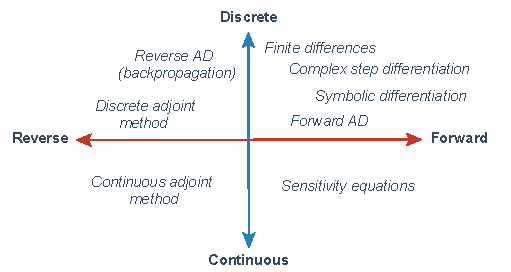
\includegraphics[width=0.80\textwidth]{figures/scheme-methods.pdf}
    \caption{Schematic representation of the different methods available for differentiation involving differential equation solutions. These can be classified depending if they find the gradient by solving a new system of differential equations (\textit{continuous}) or if instead they manipulate unit algebraic operations (\textit{discrete}). Furthermore, depending on if these methods run in the same direction as the numerical solver, we are going to be talking about \textit{backward} and \textit{forward} methods.}
    \label{fig:diff}
\end{figure}
Depending on the number of parameters and the complexity of the differential equation we are trying to solve, there are different methods to compute gradients with different numerical and computational advantages.
These methods can be roughly classified as:
\begin{itemize}
    \item \textit{Discrete} vs \textit{continuous} methods
    \item \textit{Forward} vs \textit{backward} methods
\end{itemize}
The first difference regards the fact that the method for computing the gradient can be either based on the manipulation of atomic operations that are easy to differentiate using the chain rule several times (discrete), in opposition to the approach of approximating the gradient as the numerical solution of a new set of differential equations (continuous).
Another way of conceptualizing this difference is by comparing them with the discretize-differentiate and differentiate-discretize approaches \cite{bradley2013pde, Onken_Ruthotto_2020, FATODE2014, Sirkes_Tziperman_1997}.   
We can either discretize the original system of ODEs in order to numerically solve it and then define the set of adjoint equations on top of the numerical scheme; or instead define the adjoint equation directly using the differential equation and then discretize both in order to solve \cite{Giles_Pierce_2000}.

The second distinction is related to the fact that some methods compute gradients by resolving a new sequential problem that may move in the same direction as the original numerical solver - i.e. moving forward in time - or, instead, they solve a new system that goes backwards in time. 
Figure \ref{fig:diff} displays a classification of some methods under this two-fold classification. In the following section, we are going to explore more in detail these methods.

It is important to note that if all the methods we explore in this section are mathematically correct, \textit{that does not imply they are numerically stable}.
These statements applied to methods based on pure automatic differentiation as well as adjoint methods. 
We are going to explore this consideration in more detail in section \ref{sec:computational-implementation}.

\subsection{Finite differences}
The simplest way of evaluating a derivative is by computing the difference between the evaluation of the function at a given point and a small perturbation of the function. 
In the case of the function $L : \R^p \mapsto \R$, we can approximate
\begin{equation}
 \frac{dL}{d\theta_i} (\theta) = \frac{L(\theta + \varepsilon e_i ) - L(\theta)}{\varepsilon} + \mathcal O (\varepsilon),
 \label{eq:finite_diff}
\end{equation}
with $e_i$ the $i$-th canonical vector and $\varepsilon$ the stepsize. 
Even better, the centered difference scheme leads to
\begin{equation}
 \frac{dL}{d\theta_i} (\theta) 
 =
 \frac{L(\theta + \varepsilon e_i ) - L(\theta - \varepsilon e_i)}{2\varepsilon}
 + \mathcal O (\varepsilon^2).
 \label{eq:finite_diff2}
\end{equation}
% leads to a more accurate estimation of the derivative. 
While Equation \eqref{eq:finite_diff} gives the derivative to an error of magnitude $\mathcal O (\varepsilon)$, the centered differences schemes improves the accuracy to $\mathcal O (\varepsilon^2)$ \cite{ascher2008-numerical-methods}. 
Further finite difference stencils of higher order exist in the literature \cite{Fornberg1988}. 
 
However, there are a series of problems associated with finite differences when seeking to compute the gradient of $L$.
The first is due to how it scales with the dimension $p$ of parameter vector $\theta$.
Each directional derivative requires at least one extra evaluation of the loss function.
For the centered differences approach in Equation \eqref{eq:finite_diff2}, this requires a total of $2p$ function evaluations which demands solving the differential equation each time for a new set of parameters.
A second problem is rounding errors.
Every computer ultimately stores and manipulates numbers using floating point arithmetic \cite{Goldberg_1991_floatingpoint}. 
Equations \eqref{eq:finite_diff} and \eqref{eq:finite_diff2} involve the subtraction of two numbers that are very close to each other, which leads to large cancellation errors for small values of $\varepsilon$ that are amplified by the division by $\varepsilon$.
On the other hand, large values of the stepsize give inaccurate estimations of the gradient. 
Finding the optimal value of $\varepsilon$ that balances these two effects is sometimes known as the \textit{stepsize dilemma}, for which algorithms based on prior knowledge of the function to be differentiated or algorithms based on heuristic rules have been introduced \cite{mathur2012stepsize-finitediff, BARTON_1992_finite_diff, SUNDIALS-hindmarsh2005sundials}. 
% \todo{Would be nice to show more formally the effect of the round-off error, see e.g. https://book.sciml.ai/notes/08-Forward-Mode_Automatic_Differentiation_(AD)_via_High_Dimensional_Algebras/}
% Some of these methods require some prior knowledge of the function to be differentiated, and others are based on heuristic rules. 
If well many analytical functions, like polynomials and trigonometric functions, can be computed with machine precision, numerical solutions of differential equations have errors that are typically larger than machine precision, which leads to inaccurate estimations of the gradient when $\varepsilon$ is too small. 
We will further emphasize this point in Section \ref{sec:computational-implementation}.

Despite all these caveats, finite differences can be useful when computing Jacobian-vector products (JVPs). 
Given a Jacobian matrix $J = \frac{\partial f}{\partial u}$ (or the sensitivity $s = \frac{\partial u}{\partial \theta}$) and a vector $v$, the product $Jv$ corresponding to the directional derivative and can be approximated as 
\begin{equation}
    Jv \approx \frac{f(u + \varepsilon v, \theta, t) - f(u, \theta, t)}{\varepsilon}
\end{equation}
This approach is used in numerical solvers based on Krylov methods, where linear systems are solved by iteratively solving matrix-vectors products \cite{Ipsen_Meyer_1998}.

% Replacing derivatives by finite differences is also a common practice when solving partial differential equations (PDEs), a technique known as the \textit{method of lines} \cite{ascher2008numerical}. 
% To illustrate this point, let us consider the case of the one-dimensional heat equation
% \begin{equation}
%  \frac{\partial u}{\partial t}
%  = 
%  D \, 
%  \frac{\partial^2 u}{\partial x^2}, 
%  \quad u(0, t) = \alpha(t), 
%  \quad u(1, t) = \beta(t)
%  \label{eq:heat-equation}
% \end{equation}
% that includes both spatial and temporal partial derivatives of the unknown function $u(x, t)$.
% In order to numerically solve this equation, we can define a spatial grid with coordinates $m \Delta x$, $m=0, 1, 2, \ldots, N$ and $\Delta x = 1 / N$.
% If we call $u_m(t) = u(m \Delta x, t)$ the value of the solution evaluated in the fixed points in the grid, then we can replace the second order partial derivative in Equation \eqref{eq:heat-equation} by the corresponding second order finite difference\footnote{Since $u_m(t)$ is a function of one single variable, we write the total derivative $\frac{du_m}{dt}$ instead of the partial derivative symbol used before $\frac{\partial u}{\partial t}$, which it is usually used just for multivariable function.}
% \begin{equation}
%  \frac{d u_m}{dt} 
%  = 
%  D 
%  \frac{u_{m-1} - 2u_m + u_{m+1}}{\Delta x^2}
%  \label{eq:heat-equation-discrete}
% \end{equation}
% for $m = 1, 2, \ldots, N-1$ (in the extremes we simply have $u_0(t) = \alpha(t)$ and $u_N(t)=\beta(t)$).
% Now, equation \eqref{eq:heat-equation-discrete} is a system of ordinary differential equations (just temporal derivatives) with a total of $N-1$ equations.
% This can be solved directly using an ODE solver.
% Further improvements can be made by exploiting the fact that the coupling between the different functions $u_m$ is sparse, that is, the temporal derivative of $u_m$ just depends of the values of the function in the neighbour points in the grid.



% \subsection{Complex step differentiation}
% An alternative to finite differences that avoids rounding errors is based complex variable analysis. 
The first proposals originated in 1967 using the Cauchy integral theorem involving the numerical evaluation of a complex valued integral \cite{Lyness_1967, Lyness_Moler_1967} .
A new approach recently emerged that uses the Taylor expansion of a function to define its complex generalization \cite{Squire_Trapp_1998_complex_diff}. 
Assuming that we have one single scalar parameter $\theta \in \R$, then the function $L(\theta)$ can be expanded as 
the Taylor expansion
\begin{equation}
    L(\theta + i \, \varepsilon)
    = 
    L(\theta) + i \varepsilon L'(\theta) 
    - 
    \frac 1 2
    L''(\theta) \varepsilon^2
    + 
    \mathcal O (\varepsilon^3),
\end{equation}
where $i$ is the imaginary unit with the property $i^2 = -1$. 
From this equation we can observed that many factors vanish when we compute the imaginary part $\text{Im}(L(\theta + i \varepsilon))$, which leads to
\begin{equation}
    L'(\theta) 
    = 
    \frac{\text{Im}(L(\theta + i \varepsilon))}{\varepsilon}
    + 
    \mathcal{O} (\varepsilon^2)
\end{equation}
The method of \textit{complex step differentiation} consist then in estimating the gradient as $\text{Im}(L(\theta + i \varepsilon)) / \varepsilon$ for a small value of $\varepsilon$. 
Besides the advantage of being a method with precision $\mathcal{O}(\varepsilon^2)$, the complex step method avoids subtracting cancellation error and then the value of $\varepsilon$ can be reduce to almost machine precision error without affecting the calculation of the derivative. 

Extension to higher order derivatives can be done by introducing multicomplex variables \cite{Lantoine_Russell_Dargent_2012}. 

Other authors had suggested to use complex variable analysis to compute the derivative as the imaginary part of $L(\theta + i \varepsilon)/h$, which coincides with $L'(\theta)$ for the case where $\theta$ is a scalar \cite{ Martins_Sturdza_Alonso_2003_complex_differentiation}.
% This approach was later generalized to the multivariable case 
Although this solves the problem of cancellation errors in Equation \eqref{eq:finite_diff2} for small $\varepsilon$, this approach is just valid for cases where the function $L$ is known analytically. 


\subsection{Automatic differentiation}
% I think I need some historical reference here.
Automatic differentiation (AD) is a technology that allows computing gradients thought a computer program \cite{griewank2008evaluatingderivatives}. 
The basis of all AD system is the notion that complicated functions included in any computer program can be reduced to a sequence of simple algebraic operations that have straightforward derivative expressions, based upon elementary rules of differentiation \cite{juedes1991taxonomy}.
The derivatives of the outputs of the computer program with respect to their inputs are then combined using the chain rule.
One advantage of AD systems is that we can automatically differentiate programs that include control flow, such as branching, loops or recursions. 
This is because at the end of the day, any program can be reduced to a trace of input, intermediate and output variables \cite{Baydin_Pearlmutter_Radul_Siskind_2015}.

Depending if the concatenation of these gradients is done as we execute the program (from input to output) or in a later instance were we trace-back the calculation from the end (from output to input), we are going to talk about \textit{forward} or \textit{reverse} AD, respectively.
Neither forward or reverse mode is more efficient in all cases \cite{Griewank_1989}, as we will discuss in Section \ref{sec:vjp-jvp}.

\subsubsection{Forward mode}

Forward mode AD can be implemented in different ways depending on the data structures we use at the moment of representing a computer program. Examples of these data structures include dual numbers and Wengert lists (see \cite{Baydin_Pearlmutter_Radul_Siskind_2015} for a good review on these methods). 

\vspace*{10px}
\noindent \textbf{\textit{Dual numbers}}
\vspace*{5px}

Dual numbers extend the definition of a numerical variable that takes a certain value to also carry information about its derivative with respect to certain parameter \cite{clifford1871dualnumbers}. 
We can define an abstract type, defined as a dual number, composed of two elements: a \textit{value} coordinate $x_1$ that carries the value of the variable and a \textit{derivative} coordinate $x_2$ with the value of the derivative $\frac{\partial x_1}{\partial \theta}$. 
Just as complex number, we can represent dual numbers as an ordered pair $(x_1, x_2)$, sometimes known as Argand pair, or in the rectangular form 
\begin{equation}
 x_\epsilon = x_1 + \epsilon \, x_2
\end{equation}
where $\epsilon$ is an abstract number called a perturbation or tangent, with the properties $\epsilon^2 = 0$ and $\epsilon \neq 0$.
This last representation is quite convenient since it naturally allow us to extend algebraic operations, like addition and multiplication, to dual numbers \cite{Karczmarczuk2001}. 
For example, given two dual numbers $x_\epsilon = x_1 + \epsilon x_2$ and $y_\epsilon = y_1 + \epsilon y_2$, it is easy to derive using the fact $\epsilon^2=0$ that
\begin{equation}
 x_\epsilon + y_\epsilon = (x_1 + y_1) + \epsilon \, (x_2 + y_2)
 \qquad
 x_\epsilon y_\epsilon = x_1 y_1 + \epsilon \, (x_1 y_2 + x_2 y_1) .
 %\qquad
 %\frac{x_\epsilon}{y_\epsilon} = \frac{x_1}{y_1} + \epsilon \, \frac{x_2 y_1 - x_1 y_2}{y_1^2}.
\end{equation}
From these last examples, we can see that the derivative component of the dual number carries the information of the derivatives when combining operations.
For example, suppose than in the last example the dual variables $x_2$ and $y_2$ carry the value of the derivative of $x_1$ and $x_2$ with respect to a parameter $\theta$, respectively. 

Intuitively, we can think about $\epsilon$ as being a differential in the Taylor expansion:
\begin{align}
    f(x_1 + \epsilon x_2)
    &= 
    f(x_1)
    + 
    \epsilon \, x_2 \,  f'(x_1)
    + 
    \epsilon^2 \cdot ( \ldots ) \nonumber \\
    &= 
    f(x_1)
    + 
    \epsilon \, x_2 \,  f'(x_1)
    \label{eq:dual-number-function}
\end{align}
When computing first order derivatives, we can ignore everything of order $\epsilon^2$ or larger, which is represented in the condition $\epsilon^2 = 0$.
This implies that we can use dual numbers to implement forward AD through a numerical algorithm. 
In Section \ref{sec:computational-implementation} we will explore how this is implemented and compare this approach with complex-step differentiation. 

\vspace*{10px}
\noindent \textbf{\textit{Computational graph}}
\vspace*{5px}

A useful way of representing a computer program is via a computational graph with intermediate variables that relate the input and output variables. 
Most scalar functions of interest can be represented in this factorial form as a acyclic directed graph with nodes associated to variables and edges to atomic operations \cite{griewank2008evaluatingderivatives, Griewack-on-AD}, known as Kantorovich graph \cite{kantorovich1957mathematical} or Wengert trace/tape\cite{Wengert_1964, Bauer_1974}. 
% Although notation can be a little bit difficult to digest here, the mathematics behind is rather simple. 
We can define $v_1, v_2, \ldots, v_p = \theta_1, \theta_2, \ldots, \theta_p$ the input set of variables; $v_{p+1}, \ldots, v_{m-1}$ the set of all the intermediate variables, and finally $v_m = L(\theta)$ the final output of a computer program. 
This can be done in such a way that the order is strict, meaning that each variable $v_i$ is computed just as a function of the previous variables $v_j$ with $j < i$. 
Once the graph is constructed, we can compute the derivative of every node with respect to other (a quantity known as the tangent) using Bauer formula \cite{Bauer_1974, Oktay_randomized-AD}
\begin{equation}
    \frac{\partial v_j}{\partial v_i}
    = 
    \sum_{\substack{ \text{paths }w_0 \rightarrow w_1 \rightarrow \ldots \rightarrow w_K \\
                    \text{with } w_0=v_i, w_K = v_j}}
    \prod_{k=0}^{K-1} \frac{\partial w_{k+1}}{\partial w_{k}},
\end{equation}
where the sum is calculated with respect to all the directed paths in the graph connecting the input and target node.
Instead of evaluating the last expression for all possible path, a simplification is to increasingly evaluate $j=p+1, \ldots, m$ using the recursion 
\begin{equation}
    \frac{\partial v_j}{\partial v_i}
    = 
    \sum_\text{$w$\text{ such that} $w \rightarrow v_j$}
    \frac{\partial v_j}{\partial w}
    \frac{\partial w}{\partial v_i} 
    \label{eq:AD-graph-recursion}
\end{equation}
Since every variable node $w$ such that $w \rightarrow v_j$ is an edge of the computational graph have index less than $j$, we can iterate this procedure as we run the computer program and solve for both the function and its gradient.
This is possible because in forward mode the term $\frac{\partial w}{\partial v_i}$ has been computed in a previous iteration, while $\frac{\partial v_j}{\partial w}$ can be evaluated at the same time the node $v_j$ is computed based on only the value of the parent variable nodes. 
The only requirement for differentiation is being able to compute the derivative/tangent of each edge/primitive and combine these using the recursion \eqref{eq:AD-graph-recursion}.

\subsubsection{Backward mode}

Backward mode AD is also known as the adjoint of cotangent linear mode or backpropagation in the field of machine learning. 
The reverse mode of automatic differentiation has been introduced in different contexts \cite{griewank2012invented} and materializes the observation made by Phil Wolfe that if the chain rule is implemented in reverse mode, then the ratio between the computation of the gradient of a function and the function itself can be bounded by a constant that do not depend of the number of parameters to differentiate \cite{Griewack-on-AD, Wolfe_1982}, a point known as \textit{cheap gradient principle} \cite{griewank2012invented}.  
Given a directional graph of operations defined by a Wengert list \cite{Wengert_1964}, we can compute gradients of any given function in the same fashion as Equation \eqref{eq:AD-graph-recursion} but in backwards mode as
\begin{equation}
 \bar v_i = \frac{\partial \ell}{\partial v_i}= \sum_{w : v \rightarrow w \in G} \frac{\partial w}{\partial v} \bar{w}.
\end{equation}
Here we have introduced the notation $\bar{\omega} = \frac{\partial \ell}{\partial \omega}$ to indicate that the partial derivative is always of the final loss function with respect to the different program variables, a quantity sometimes refers as adjoint (do not confuse with the adjoint method of later sections) or cotangent. 
Since in backwards AD the values of $\bar \omega$ are being updated in reverse order, in order to evaluate the terms $\frac{\partial \omega}{\partial v}$ we need to know the state value of all the argument variables $v$ of $\omega$, which need to be stored in memory during the evaluation of the function in order to be able to apply backward AD.


\subsubsection{AD connection with JVPs and VJPs}
\label{sec:vjp-jvp}

When working with unit operations that involve matrix operations dealing with vectors of different dimensions, the order in which we apply the chain rule matters \cite{Giering_Kaminski_1998}.
When computing a gradient using AD, we can encounter vector-Jacobian products (VJPs) or Jacobian-vector products (JVP).
As their name indicates, the difference between them regards the fact that the quantity we are interested in computing is described by the product of a Jacobian by a vector on the left side (VJP) or the right (JVP).

For nested functions, the Jacobian is described as the product of multiple Jacobians using the chain rule.
In this case, the full gradient is computed as the chain product of vectors and Jacobians. 
Let us consider for example the case of a loss function $L : \mathbb R^p \mapsto \mathbb R$ taking a total of $p$ arguments as inputs that can be decomposed as $L(\theta) = \ell \circ g_{k} \circ \ldots \circ g_2 \circ g_1(\theta)$, with $\ell : \mathbb R^{d_k} \mapsto \mathbb R$ the final evaluation of the loss function after we apply in order a sequence of intermediate functions $g_i : \mathbb R^{d_{i-1}} \mapsto \mathbb R^{d_i}$, where we define $d_0 = p$ for simplicity. 
Using the chain rule states that the gradient of the final loss function is
\begin{equation}
 \nabla_\theta L = \nabla \ell \cdot Dg_{k} \cdot Dg_{k-1} \cdot \ldots \cdot Dg_2 \cdot Dg_1, 
\end{equation}
with $Dg_i$ the Jacobians of each nested function. 
Notice that in the last equation, $\nabla \ell \in \mathbb R^{d_k}$ is a vector.
In order to compute $\nabla_\theta L$, we can solve the multiplication starting from the right side, which will correspond to multiplying the Jacobians forward from $Dg_1$ to $Dg_k$, or from the left side, moving backwards. 
The important aspect of the backwards case is that we will always be computing VJPs, since $\nabla \ell$ is a vector.
Since VJPs are easier to evaluate than full Jacobians, the backward mode will be in general faster when $1 \ll p$.
To illustrate this, let us consider the following example displayed in Figure \ref{fig:vjp-jvp}. 
For general rectangular matrices $A\in \mathbb R^{d_1 \times d_2}$ and $B \in \mathbb R^{d_2 \times d_3}$, the cost of the matrix multiplication $AB$ is $\mathcal O (d_1 d_2 d_3)$.
It is worth noticing that if well more efficient methods for matrix-matrix multiplication based on Strassen’s recursive algorithm and its variants exist, these are not extensively used in most scientific applications \cite{Silva_Gustafson_Wong_2018, Huang_Smith_Henry_Geijn_2016}.
This implies that forward AD requires a total of
\begin{equation}
 d_2 d_1 p + d_3 d_2 p + \ldots + d_k d_{k-1} p + d_k p = \mathcal O (kp)
\end{equation}
operations, while backwards mode AD requires
\begin{equation}
 d_k d_{k-1} + d_{k-1} d_{k-2} + \ldots + d_2 d_1 + d_1 p = \mathcal O (k+p)
\end{equation}
operations, where the $\mathcal O$ is with respect to the variable $p$. 

In the general case of a function $L : \R^p \mapsto \R^q$ with multiple outputs and a total of $k$ intermediate functions, the cost of forward AD is $\mathcal O (pk + q)$ and the cost of reverse is $\mathcal O (p + kq)$.
When the function to differentiate has a larger input space than output ($q \ll p$), AD in backward mode is more efficient as it propagates the chain rule by computing VJPs, the reason why backwards AD is more used in modern machine learning.
% On the other side, when the output dimension is larger than the input space dimension, forwards AD is more efficient.
% This is the reason why in most machine learning application people use backwards AD. 
However, notice that backwards mode AD requires us to save intermediate variables through the forward run in order to run backwards afterwards \cite{Bennett_1973}, leading to performance overhead that makes forward AD more efficient when $p \lesssim q$ \cite{Griewank_1989, Margossian_2018, Baydin_Pearlmutter_Radul_Siskind_2015}.  
In other words, backwards AD is really more efficient when $q \ll p$. 
% while in forward mode we can just evaluate the gradient as we iterate our sequence of functions. 
This problem can be mitigated, to some extent, with a good checkpointing scheme we will discuss later. 
% On the other hand, when the goal is to compute the gradient of many function outputs with respect to a few parameters, forward mode AD is more efficient \cite{Griewank_1989}.
% This means that for problems with a small number of parameters, forward mode can be faster and more memory-efficient that backwards AD.

\begin{figure}[t]
    \centering
    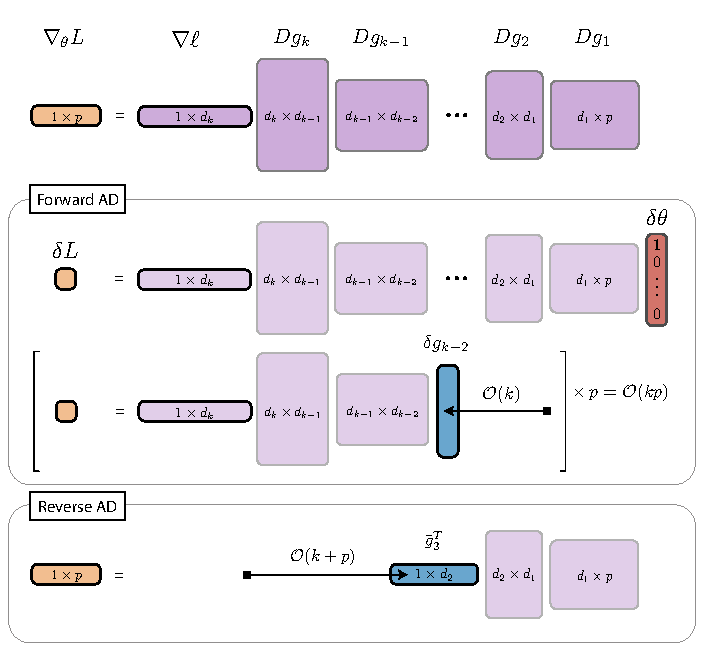
\includegraphics[width=0.95\textwidth]{tex/figures/VJP-AD.pdf}
    \caption{Comparison between forward and backward AD. Changing the order of how we multiply the Jacobians change the total number of floating-point operations, which leads to different computational complexities between forward and backward mode. When the multiplication is carried from the right side of the mathematical expression for $\nabla_\theta L$, each matrix simplification involves a matrix with size $p$, giving a total complexity of $\mathcal O (kp)$. This is the opposite of what happens when we carried the VJP from the left side of the expression, where the matrix of size $d_1 \times p$ has not affect in the intermediate calculations, making all the intermediate calculations $\mathcal O (1)$ with respect to $p$ and a total complexity of $\mathcal O (k + p)$. }
    % However, backwards mode requires storing in memory information about the forward execution of the program, while forward mode can update the gradient on running time.}
    \label{fig:vjp-jvp}
\end{figure}


\subsection{Sensitivity equations}
An easy way to derive an expression for the sensitivity $s$ defined in Equation \eqref{eq:sensitivity-definition} is by deriving the forward sensitivity equations \cite{ramsay2017dynamic}, a method also referred to as continuous local sensitivity analysis (CSA). 
If we consider the original ODE given by Equation \eqref{eq:original_ODE} and we differentiate with respect to $\theta$, we then obtain
\begin{equation}
    \frac{d}{d\theta} \left( \frac{du}{dt}  - f(u(\theta), \theta, t) \right) = 0.
\end{equation}
Assuming that a unique solution exists and both $\frac{\partial f}{\partial u}$ and $\frac{\partial f}{\partial \theta}$ are continuous in the neighbourhood of the solution, or under the guarantee of interchangeability of the derivatives \cite{gronwall1919note}, for example by assuming that both $\frac{du}{dt}$ and $\frac{du}{d\theta}$ are differentiable \cite{math8111947}, we can derive
\begin{equation}
 \frac{d}{d\theta} \frac{du}{dt} 
 =
 \frac{d}{d\theta} f(u(\theta), \theta, t)
 = 
 \frac{\partial f}{\partial \theta}
 + 
 \frac{\partial f}{\partial u} \frac{\partial u}{\partial \theta}.
\end{equation}
Identifying the sensitivity matrix $s(t)$ now as a function of time, we obtain the \textit{sensitivity differential equation} 
\begin{equation}
 \frac{ds}{dt} = \frac{\partial f}{\partial u} s + \frac{\partial f}{\partial \theta}.
 \label{eq:sensitivity_equations}
\end{equation}
The initial condition is simply given by $s(t_0) = \frac{du_0}{d\theta}$, which is zero unless the initial condition explicitly depends on the parameter $\theta$.
Both the original ODE of size $n$ and the forward sensitivity equation with size $np$ are solved simultaneously, which is necessary since the forward sensitivity DE directly depends on the value of $u(t)$.  
This implies that as we solve the ODE, we can ensure the same level of numerical precision for the two of them inside the numerical solver.

In contrast to the methods previously introduced, the forward sensitivity equations find the derivative by solving a new set of continuous differential equations.
Notice also that the obtained sensitivity $s(t)$ can be evaluated at any given time $t$. 
This method can be labeled as forward, since we solve both $u(t)$ and $s(t)$ as we solve the DE forward in time, without the need of backtracking any operation though the solver.
By solving the forward sensitivity equation and the original ODE for $u(t)$ simultaneously, we ensure that by the end of the forward step we have calculated both $u(t)$ and $s(t)$. 

\subsection{Discrete adjoint method}
Also know as the adjoint state method, it is another example of a discrete method that aims to find the gradient by solving an alternative system of linear equations, known as the \textit{adjoint equations}, at the same time that we solve the original system of linear equations defined by the numerical solver. 
These methods are extremely popular in optimal control theory in fluid dynamics, for example for the design of geometries for vehicles and airplanes that optimize performance \cite{Elliott_Peraire_1996, Giles_Pierce_2000}.
This approach follows the discretize-optimize approach, meaning that we first discretize the system of continuous ODEs and then solve on top of these linear equations \cite{Giles_Pierce_2000}. 

% Just as in the case of automatic differentiation, the adjoint state method evaluates the gradient by moving forward in time and applying the chain rule sequentially over a discrete set of operations that dictate the updates by the numerical scheme for solving the differential equation. However, it does so by directly computing the gradient by solving a new system of equations.

% Mathematically, reverse mode AD is related to the adjoint differential equations \cite{Griewack-on-AD}

\vspace*{10px}
\noindent \textbf{\textit{Discrete differential equation}}
\vspace*{5px}

% reference: Sensitivity theory of non-linear systems

The first step in order to derive the adjoint equation is to discretize the ODE in Equation \eqref{eq:original_ODE} into finite evaluations of the function $u(t; \theta)$. 
Given the sequence of timesteps $t_0, t_1, \ldots, t_N$, we evaluate the solution at $u_i = u(t_i; \theta)$. 
Most commonly used numerical solver consists in linear multisteps methods with the form 
\begin{equation}
    \sum_{i=1}^{K_1} \alpha_{n,i} u_{n-i} 
    +
    h_n \sum_{i=1}^{K_2} \beta_{n,i} f(u_{n-i}, \theta, t_i)
    = 
    0
\end{equation}
In the case of using an explicit numerical solver, these values will be constrained to satisfy a set of equations of the form 
\begin{equation}
    u_{i+1} = A_i (\theta) \, u_i + b_i
\end{equation}
with $A_i \in \R^{n \times n}$ a squared matrix defined by the numerical solver. 
Solving the differential equation then implies to be able to solve the system of constraints 
\begin{equation}
    g_i (u_{i+1}; \theta) = u_{i+1} - A_i (\theta) \, u_i - b_i = 0
\end{equation}
for all $i=0, 1, \ldots, N-1$. 
For most cases, this system can be solved sequentially, by solving for $u_i$ in increasing order of index. 
If we call the super-vector $U = (u_1, u_2, \ldots, u_N) \in \R^{nN}$, we can combine all these equations in into one single system of linear equations 
\begin{equation}
    A(\theta) U 
    = 
    \begin{bmatrix}
        \I_{n \times n} & 0 &   &  & \\
        -A_1 & \I_{n \times n} & 0 &  &  \\
          & -A_2 & \I_{n \times n} & 0 &  \\
         &  &   & \ddots &   \\
         &  &  & -A_{N-1} & \I_{n \times n}
    \end{bmatrix}
    \begin{bmatrix}
        u_1 \\
        u_2 \\
        u_3 \\
        \vdots \\
        u_N
    \end{bmatrix}
    = 
    \begin{bmatrix}
        A_0 u_0 + b_0 \\
        b_1 \\
        b_2 \\
        \vdots \\
        b_{N-1}
    \end{bmatrix}
    = 
    b(\theta), 
\end{equation}
with $\I_{n \times n}$ the identity matrix of size $n \times n$.
It is usually convenient to write this system of linear equations in the residual form $G(U; \theta) = 0$, where $G(U; \theta) = A(\theta) U - b(\theta)$ is the residual between both sides of the equation. 
Different numerical schemes will lead to different design matrix $A(\theta)$ and vector $b(\theta)$, but ultimately every numerical method will lead to a system of linear equations with the form $G(U; \theta) = A(\theta) U - b(\theta) = 0$ after being discretized. 
It is important to notice that in most cases, the matrix $A(\theta)$ is quite large and mostly sparse. 
If well this representation of the discrete differential equation is quite convenient for mathematical manipulations, at the moment of solving the system we will rely in iterative solvers that save memory and computation. 

\vspace*{10px}
\noindent \textbf{\textit{Adjoint state equations}}
\vspace*{5px}

We are interested in differentiating a function $L(U, \theta)$ with respect to the parameter $\theta$. 
Since here $U$ is the discrete set of evaluations of the solution, examples of loss functions now include 
\begin{equation}
    L(U, \theta) 
    = 
    \frac{1}{2} \sum_{i=1}^N \| u_i - u_i^\text{obs} \|^2, 
\end{equation}
with $u_i^\text{obs}$ the observed time-series. 
We further need to impose the constraint that the solution satisfies the algebraic linear equation $G(U; \theta) = 0$.
Now,
\begin{equation}
    \frac{dL}{d\theta} 
    = 
    \frac{\partial L}{\partial \theta} 
    + 
    \frac{\partial L}{\partial U} \frac{\partial U}{\partial \theta},
    \label{eq:dhdtheta0}
\end{equation}
and also for the constraint $G(U; \theta)=0$ we can derive
\begin{equation}
    \frac{dG}{d\theta} 
    = 
    \frac{\partial G}{\partial \theta} 
    + 
    \frac{\partial G}{\partial U} \frac{\partial U}{\partial \theta}
    =
    0
\end{equation}
which is equivalent to 
\begin{equation}
    \frac{\partial U}{\partial \theta} 
    = 
    - \left( \frac{\partial G}{\partial U} \right)^{-1} \frac{\partial G}{\partial \theta}.
\end{equation}
If we replace this last expression into equation \eqref{eq:dhdtheta0}, we obtain
\begin{equation}
    \frac{dL}{d\theta} 
    =
    \frac{\partial L}{\partial \theta} 
    - 
    \underbrace{\frac{\partial L}{\partial U}}_{\text{vector}}
    \left( \frac{\partial G}{\partial U} \right)^{-1} 
    \frac{\partial G}{\partial \theta}.
    \label{eq:dhdtheta}
\end{equation}
The important trick in the adjoint state methods is to observe that in this last equation, the right-hand side can be resolved as a vector-Jacobian product (VJP).
Instead of computing the product of the matrices $\left( \frac{\partial G}{\partial U} \right)^{-1}$ and $\frac{\partial G}{\partial \theta}$, it is computationally more efficient first to compute the resulting vector from the operation $\frac{\partial L}{\partial U} \left( \frac{\partial G}{\partial U} \right)^{-1}$ and then multiply this by $\frac{\partial G}{\partial \theta}$.
This is what leads to the definition of the adjoint $\lambda \in \R^{nN}$ as the solution of the linear system of equations 
\begin{equation}
    \left( \frac{\partial G}{\partial U}\right)^T \lambda 
    =  
    \left( \frac{\partial L}{\partial U} \right)^T,
    \label{eq:adjoint-state-equation}
\end{equation}
that is,
\begin{equation}
    \lambda^T = \frac{\partial L}{\partial U} \left( \frac{\partial g}{\partial U} \right)^{-1}.
    \label{eq:def_adjoint}
\end{equation}
Finally, if we replace Equation \eqref{eq:def_adjoint} into \eqref{eq:dhdtheta}, we obtain 
\begin{equation}
    \frac{dL}{d\theta} 
    =
    \frac{\partial L}{\partial \theta} 
    - 
    \lambda^T \frac{\partial G}{\partial \theta}.
    \label{eq:gradient-adjoint-state-method}
\end{equation}
The important trick to notice here is the rearrangement of the multiplicative terms involved in equation \eqref{eq:dhdtheta}. Computing the full Jacobian/sensitivity $\partial u / \partial \theta$ will be computationally expensive and involves the product of two matrices. However, we are not interested in the calculation of the Jacobian, but instead in the VJP given by $\frac{\partial L}{\partial U} \frac{\partial U}{\partial \theta}$. By rearranging these terms, we can make the same computation more efficient. 

For the linear system of discrete equations $G(U; \theta)=0$, we have \cite{Johnson}
\begin{equation}
    \frac{\partial G}{\partial \theta} 
    = 
    \frac{\partial A }{\partial \theta} U - \frac{\partial b}{\partial \theta},
\end{equation}
so the desired gradient in Equation \eqref{eq:gradient-adjoint-state-method} can be computed as 
\begin{equation}
    \frac{dL}{d\theta} 
    = 
    \frac{\partial L}{\partial \theta} 
    - 
    \lambda^T \left( \frac{\partial A }{\partial \theta} U - \frac{\partial b}{\partial \theta} \right)
    \label{eq:dhdtheta_linear}
\end{equation}
with $\lambda$ the solution of the linear system (Equation \eqref{eq:adjoint-state-equation})
\begin{equation}
    A(\theta)^T \lambda 
    =
    \begin{bmatrix}
        \I_{n \times n} & -A_1^T &   &  & \\
        0 & \I_{n \times n} & -A_2^T &  &  \\
          & 0 & \I_{n \times n} & -A_3^T &  \\
         &  &   & \ddots & -A_{N-1}^T  \\
         &  &  & 0 & \I_{n \times n}
    \end{bmatrix}
    \begin{bmatrix}
        \lambda_1 \\
        \lambda_2 \\
        \lambda_3 \\
        \vdots \\
        \lambda_N
    \end{bmatrix}
    = 
    \begin{bmatrix}
        u_1 - u_1^\text{obs} \\
        u_2 - u_2^\text{obs} \\
        u_3 - u_3^\text{obs} \\
        \vdots \\
        u_N - u_N^\text{obs}     
    \end{bmatrix}
    = 
    \frac{\partial L}{\partial U}^T.
    \label{eq:linea-adjoint-state-equation}
\end{equation}
This is a linear system of equations with the same size of the original $A(\theta) U = b(\theta)$, but involving the adjoint matrix $A^T$. 
Computationally this also means that if we can solve the original system of discretized equations then we can also solve the adjoint. 
One way of doing this is relying on matrix factorization. 
Using the LU factorization we can write the matrix $A(\theta)$ as the product of a lower and upper triangular matrices $A (\theta) = LU$, which then can be also used for solving the adjoint equation since $A^T(\theta)=U^TL^T$.
Another more natural way of finding the adjoins $\lambda$ is by noticing that the system of equations \eqref{eq:linea-adjoint-state-equation} is equivalent to the iterative scheme
\begin{equation}
    \lambda_{i} = A_{i}^T \lambda_{i+1} + (u_i - u_i^\text{obs})
\end{equation}
with initial condition $\lambda_N$. 
This means that we can solve the adjoint equation in backwards mode, starting from the final state $\lambda_N$ and computing the values of $\lambda_i$ in decreasing index order. 
In principle, notice that in order to do this we need to know the value of $u_i$ at any given timestep. 
% When do we solve this backwards and when forward?


%In order to compute the gradient of the full solution of the differential equation, we apply this method sequentially using the chain rule. One single step of the state method can be understood as the chain of operations $\theta \mapsto g \mapsto u \mapsto L$. This allows us to create adjoints for any primitive function $g$ (i.e. the numerical solver scheme) we want, and then incorporated it as a unit of any AD program. 

% \subsubsection{Further remarks}

% Conection with duality
% Conection with the adjoint operator
% Different ways of deriving the adjoint equations: lagrangian
% Is the adjoint the same than a gradient? Yes, but these are derivatives with respect to the state of the system, not with respect to the parameters! 

\subsection{Continuous adjoint method}
The continuous adjoint method, also known as continuous adjoint sensitivity analysis (CASA), operates by defining a convenient set of new differential equations for the adjoint variable and using this to compute the gradient in a more efficient manner. 
We encourage the interested reader to make the effort of following how the continuous adjoint method follows the same logic than the discrete adjoint method, but where the discretization of the differential equation does not happen until the very last step, when the solutions of the differential equations involved need to be numerically evaluated. 
The Lagrangian derivation of the continuous adjoint method can also be found in Appendix \ref{appendix:lagrangian}.
%\footnote{Based on slides of Chris Rackauckas about "Data Efficient model discovery with Scientific Machine Learning", Neural ODE paper, video "The use and practice of scientific machine learning". Paper comparing CSA and DSA} 

Consider an integrated loss function defined in Equation \eqref{eq:integrated-loss-function} of the form 
\begin{equation}
    L(u; \theta) = \inttime h(u(t;\theta), \theta) dt
\end{equation}
and its derivative with respect to the parameter $\theta$ given by the following integral involving the sensitivity matrix $s(t)$:
\begin{equation}
    \frac{dL}{d\theta}
    = 
    \inttime \left( \frac{\partial h}{\partial \theta} + \frac{\partial h}{\partial u} s(t) \right) dt.
    \label{eq:casa-loss}
\end{equation}
Just as in the case of the discrete adjoint method, the complicated term to evaluate in the last expression is the sensitivity (Equation \eqref{eq:sensitivity-definition}).
Again, the trick is to evaluate the VJP $\frac{\partial h}{\partial u} \frac{\partial u}{\partial \theta}$ by first defining an intermediate adjoint variable. 
The continuous adjoint equation now is obtained by finding the dual/adjoint equation of the sensitivity equation using the weak formulation of Equation \eqref{eq:sensitivity_equations}. 
The adjoint equation is obtained by writing the sensitivity equation in the form 
\begin{equation}
    \inttime \lambda(t)^T \left( \frac{ds}{dt} - f(u, \theta, t) \, s - \frac{\partial f}{\partial \theta}  \right) dt 
    = 
    0,
    \label{eq:integrated-sensitivity-equation}
\end{equation}
where this equation must be satisfied for every function $\lambda(t)$ in order for Equation \eqref{eq:continuous-adjoint} to be true. 
The next step is to get rid of the time derivative applied to the sensitivity $s(t)$ using integration by parts: 
\begin{equation}
    \inttime \lambda(t)^T \frac{ds}{dt} dt
    = 
    \lambda(t_1)^T s(t_1) - \lambda(t_0)^T s(t_0)
    -
    \inttime \frac{d\lambda^T}{dt} s(t)\, dt.
\end{equation}
Replacing this last expression into Equation \eqref{eq:integrated-sensitivity-equation} we obtain 
\begin{equation}
    \inttime \left( - \frac{d\lambda^T}{dt} -  \lambda(t)^T f(u, \theta, t) \right) s(t) dt
    =
    \inttime \lambda(t)^T \frac{\partial f}{\partial \theta} dt 
    - 
    \lambda(t_1)^T s(t_1)
    + 
    \lambda(t_0)^T s(t_0).
    \label{eq:casa-semiadjoint}
\end{equation}
At first glance, there is nothing particularly interesting about this last equation. 
However, both Equations \eqref{eq:casa-loss} and \eqref{eq:casa-semiadjoint} involve a VJP with $s(t)$. 
Since Equation \eqref{eq:casa-semiadjoint} must hold for every function $\lambda(t)$, we can pick $\lambda(t)$ to make the terms involving $s(t)$ in Equations \eqref{eq:casa-loss} and \eqref{eq:casa-semiadjoint} to perfectly coincide. 
This is done by defining the adjoint $\lambda(t)$ to be the solution of the new system of differential equations
\begin{equation}
    \frac{d\lambda}{dt} 
    = 
    - 
    f(u, \theta, t)^T \lambda  
    - 
    \frac{\partial h^T}{\partial u} 
    \qquad \quad \lambda(t_1) = 0. 
    \label{eq:casa-adjoint-equation}
\end{equation}
Notice that the adjoint equation is defined with the final condition at $t_1$, meaning that it needs to be solved backwards in time. 
The definition of the adjoint $\lambda(t)$ as the solution of this last ODE simplifies Equation \eqref{eq:casa-semiadjoint} to
\begin{equation}
    \inttime \frac{\partial h}{\partial u} s(t) dt
    = 
    \lambda(t_0)^T s(t_0)
    + 
    \inttime \lambda(t)^T \frac{\partial f}{\partial \theta} dt.
\end{equation}
Finally, replacing this inside the expression for the gradient of the loss function we have 
\begin{equation}
    \frac{dL}{d\theta}
    = 
    \lambda(t_0)^T s(t_0)
    + 
    \inttime
    \left( \frac{\partial h}{\partial \theta} + \lambda^T \frac{\partial f}{\partial \theta} \right) dt
    \label{eq:casa-final-loss-gradient}
\end{equation}
The full algorithm to compute the full gradient $\frac{dL}{d\theta}$ can be described as follows:
\begin{enumerate}
    \item Solve the original differential equation $\frac{du}{dt} = f(u, t, \theta)$;
    \item Solve the backwards adjoint differential equation given by Equation \eqref{eq:casa-adjoint-equation};
    \item Compute the gradient using Equation \eqref{eq:casa-final-loss-gradient}.
\end{enumerate}

More general recipes for deriving continuous adjoint methods exists, including generalizations for PDEs. 
The adjoint methods can be formulated as ... 

% \subsubsection{Are discrete and continuous adjoint the same?}




\section{Comparison between methods}
% Giles (2000) has a good discussion on this.


% \section{Do we need full gradients?}

% \section{Generalization to PDEs}

% \section{Open science from scratch}

\section{Notation}
\setlength{\tabcolsep}{10pt} % Default value: 6pt
\renewcommand{\arraystretch}{1.2}
\begin{table}[H]
    \center
    \begin{tabular}{| p{3cm} | p{8cm} |}
    \hline
    Variable            & Meaning \\ [0.5ex] 
    \hline  
    $u$					& Solution of the differential equation \\
    $\theta$            & Parameters of the model \\
    $L$ 				& Loss function \\
    $s$                 & Sensitivity of the solution given by $\frac{\partial u}{\partial \theta}$ \\
    $n$                 & Number of ODEs \\
    $p$                 & Number of parameters \\
    \hline
\end{tabular}	
\end{table}


\newpage
\appendix
\section*{Appendices}
\addcontentsline{toc}{section}{Appendices}
\renewcommand{\thesubsection}{\Alph{subsection}}

\subsection{Lagrangian derivation of adjoints}
\label{appendix:lagrangian}

%by the means of the \emph{Lagrange multiplier method}\cite{Vadlamani.2020}.
% The introduction of the adjoint variable allows to reduce the computational complexity of sensitivity methods, as we will explore in this section and later in Section \ref{section:computing-adjoints}.

The adjoint equation can be derived directly from the 
Following the analysis in \cite{Giles_Pierce_2000}, we decided to present both approaches here, although we prefer with the duality viewpoint introduced in the main text since we believe is more commonly used and easy to understand for newcomers. 

In this section we are going to derive the adjoint equation for both discrete and continuous methods using the Lagrangian formulation of the adjoint. 
It is important to mention that this is different than using the Lagrange multipliers approach, a common confusion in the literature\cite{Givoli_2021}.
Conceptually, the method is the same in both discrete and continuous case, with the difference that we manipulate linear algebra objects for the former and continuous operators for the later. 

\subsubsection{Discrete adjoint}

\subsubsection{Continuous adjoint}

For the continuous adjoint method, we proceed the same way by writing a new loss function $I(\theta)$, sometimes known as the \textit{Lagrangian}, identical to $L(\theta)$ as 
\begin{equation}
    I(\theta) = L(\theta) - \inttime \lambda(t)^T \left( \frac{du}{dt} - f(u, \theta, t) \right) dt
\end{equation}
where $\lambda(t) \in \mathbb R^n$ is the Lagrange multiplier of the continuous constraint defined by the differential equation. Now, 
\begin{equation}
    \frac{dL}{d\theta} = \frac{dI}{d\theta} = 
    \inttime \left( \frac{\partial h}{\partial \theta} + \frac{\partial h}{\partial u} \frac{\partial u}{\partial \theta} \right) dt
    - 
    \inttime \lambda(t)^T \left( \frac{d}{dt} \frac{du}{d\theta} - \frac{\partial f}{\partial u} \frac{du}{d\theta} - \frac{\partial f}{\partial \theta} \right) dt.
\end{equation}
Notice that the term involved in the second integral is the same we found when deriving the sensitivity equations. 
We can derive an easier expression for the last term using integration by parts. 
Using our usual definition of the sensitivity $s = \frac{du}{d\theta}$, and performing integration by parts in the term $\lambda^T \frac{d}{dt} \frac{du}{d\theta}$ we derive 
\begin{multline}
    \frac{dL}{d\theta}
    = 
    \inttime \left( \frac{\partial h}{\partial \theta} + \lambda^T \frac{\partial f}{\partial \theta} \right) dt 
    - 
    \inttime \left( - \frac{d\lambda^T}{dt} - \lambda^T \frac{\partial f}{\partial u} - \frac{\partial h}{\partial u} \right) \, s(t) \, dt \\
    -
    \bigg ( \lambda(t_1)^T s(t_1) - \lambda(t_0)^T s(t_0) \bigg ).
    \label{eq:continous-adjoint-loss}
\end{multline}
Now, we can force some of the terms in the last equation to be zero by solving the following adjoint differential equation for $\lambda(t)^T$ in backwards mode
\begin{equation}
    \frac{d\lambda}{d\theta} = - \left(\frac{\partial f}{\partial u}\right)^T \lambda - \left( \frac{\partial h}{\partial u} \right)^T,
    \label{eq:continuous-adjoint}
\end{equation}
with final condition $\lambda(t_1) = 0$. 

It is easy to see that this derivation is equivalent to solving the Karush-Kuhn-Tucker (KKT) conditions. 

% \section{Glossary} 

\newpage
\printbibliography[heading=bibintoc, title={References}]

\end{document}
